\documentclass[12pt,a4paper]{article}

\usepackage[a4paper,margin=1in]{geometry}
\usepackage{amsmath}
\usepackage{booktabs}
\usepackage{graphicx}
\usepackage{float}
\usepackage{listings}
\usepackage{xcolor}
\usepackage{fancyhdr}
\usepackage{tikz}
\usetikzlibrary{calc}
\usepackage{array}

\pagestyle{fancy}
\fancyhf{}
\fancyfoot[C]{\thepage}

\definecolor{keyword}{RGB}{0,0,180}
\definecolor{comment}{RGB}{0,120,0}

\lstset{
basicstyle=\ttfamily\small,
keywordstyle=\color{keyword},
commentstyle=\color{comment},
frame=single,
breaklines=true,
showstringspaces=false
}

\begin{document}

%%%%%%%%%%%%%%%%%%%%%%%%%%%%%%%%%%%%%%%%%%%%%%%%%%%%%%
%%%%%%%%%%%%%%%%%%%% COVER PAGE %%%%%%%%%%%%%%%%%%%%%%
%%%%%%%%%%%%%%%%%%%%%%%%%%%%%%%%%%%%%%%%%%%%%%%%%%%%%%

\begin{titlepage}

\begin{tikzpicture}[remember picture,overlay]
\draw[line width=2pt]
($(current page.north west)+(1cm,-1cm)$)
rectangle
($(current page.south east)+(-1cm,1cm)$);
\end{tikzpicture}

\centering

\vspace{1.5cm}

{\Huge\textbf{Experiment Report}}

\vspace{0.6cm}

{\LARGE\textbf{Logic Function Realization}}

\vspace{0.3cm}

Reference: GATE EE 2019 (Question 19)

\vspace{2cm}

\renewcommand{\arraystretch}{2}

\begin{tabular}{ll}
Submitted By & : Kalpana Kumari \\
Internship & : Summer Internship, 2026 \\
Organization & : Indian Institute of Technology, Hyderabad \\
\end{tabular}

\vfill

\large
Department of Electrical Engineering

\end{titlepage}

%%%%%%%%%%%%%%%%%%%%%%%%%%%%%%%%%%%%%%%%%%%%%%%%%%%%%%

\section{Objective}

The objective of this experiment is to analyse the given combinational logic circuit from GATE EE 2019, derive its Boolean expression, verify the corresponding truth table and identify the logic function implemented by the circuit.

%%%%%%%%%%%%%%%%%%%%%%%%%%%%%%%%%%%%%%%%%%%%%%%%%%%%%%

\section{Circuit Analysis}

The given logic circuit consists of two NOT operations, two AND operations and one OR operation.

The first product term generated is

\[
T_1=\overline{X}Y
\]

The second product term generated is

\[
T_2=X\overline{Y}
\]

The final output is obtained by ORing the two product terms.

\[
Z=T_1+T_2
\]

Therefore,

\[
Z=\overline{X}Y+X\overline{Y}
\]

This expression is the standard Boolean expression of an Exclusive-OR (XOR) gate.

Hence,

\[
\boxed{Z=X\oplus Y}
\]

%%%%%%%%%%%%%%%%%%%%%%%%%%%%%%%%%%%%%%%%%%%%%%%%%%%%%%

\section{Truth Table}

\begin{table}[H]
\centering

\renewcommand{\arraystretch}{1.4}

\begin{tabular}{|c|c|c|c|c|c|c|}
\hline

$X$ &
$Y$ &
$\overline X$ &
$\overline Y$ &
$\overline XY$ &
$X\overline Y$ &
$Z$

\\
\hline

0&0&1&1&0&0&0\\
\hline

0&1&1&0&1&0&1\\
\hline

1&0&0&1&0&1&1\\
\hline

1&1&0&0&0&0&0\\
\hline

\end{tabular}

\caption{Truth table of the derived Boolean expression}

\end{table}

%%%%%%%%%%%%%%%%%%%%%%%%%%%%%%%%%%%%%%%%%%%%%%%%%%%%%%
\newpage
\section{Circuit Diagram}

The combinational logic circuit provided in the GATE EE 2019 question implements

\[
Z=\overline{X}Y+X\overline{Y}
\]

which is equivalent to an XOR gate.

\vspace{0.5cm}

\begin{figure}[H]
\centering
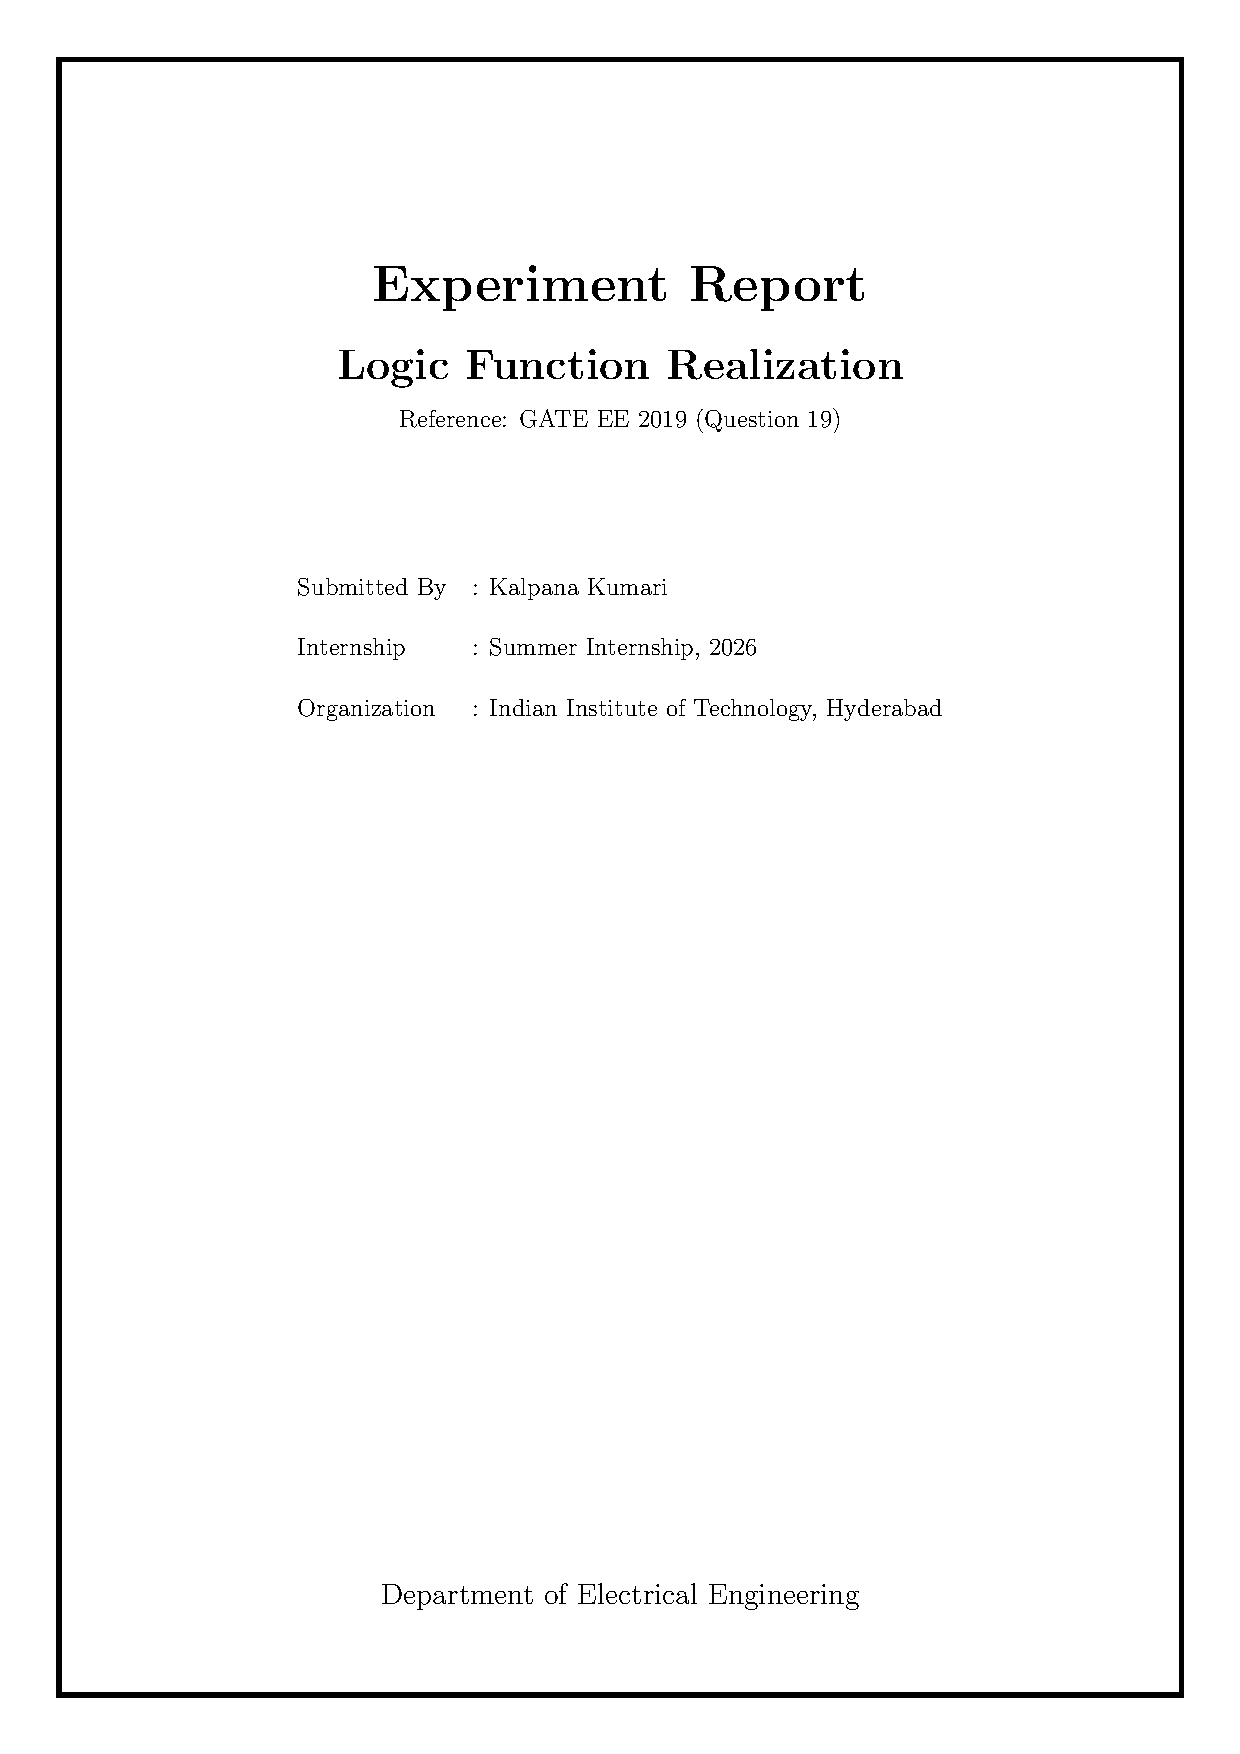
\includegraphics[width=0.8\textwidth]{gate_problem.png}
\caption{Logic circuit from GATE EE 2019 Question 19}
\end{figure}
%%%%%%%%%%%%%%%%%%%%%%%%%%%%%%%%%%%%%%%%%%%%%%%%%%%%%%

\section{Hardware Requirements}

The experiment was carried out without using any logic ICs. The following components were used:

\begin{itemize}
    \item Breadboard
    \item LEDs
    \item 330 $\Omega$ Resistors
    \item Jumper Wires
    \item 5 V DC Supply
\end{itemize}

%%%%%%%%%%%%%%%%%%%%%%%%%%%%%%%%%%%%%%%%%%%%%%%%%%%%%%

\section{Experimental Procedure}

\begin{enumerate}
    \item The breadboard was powered using a regulated 5 V supply.
    \item Two input lines ($X$ and $Y$) were connected manually using jumper wires.
    \item LEDs were used to indicate the logic levels of the inputs and output.
    \item All four input combinations were applied sequentially.
    \item The observed output was compared with the theoretical truth table.
\end{enumerate}

%%%%%%%%%%%%%%%%%%%%%%%%%%%%%%%%%%%%%%%%%%%%%%%%%%%%%%

\section{Observation}

The output LED remained OFF for input combinations (00) and (11), whereas it turned ON for (01) and (10). The observed results matched the theoretical behaviour of an XOR gate.

%%%%%%%%%%%%%%%%%%%%%%%%%%%%%%%%%%%%%%%%%%%%%%%%%%%%%%

\section{Result}

The given combinational logic circuit implements the XOR function.

\[
Z=\overline{X}Y+X\overline{Y}=X\oplus Y
\]

The practical observations verified the correctness of the derived Boolean expression.

%%%%%%%%%%%%%%%%%%%%%%%%%%%%%%%%%%%%%%%%%%%%%%%%%%%%%%

\section{Embedded C Program}

\begin{lstlisting}[language=C]
#include <avr/io.h>

int main(void)
{
    DDRB &= ~((1<<PB0) | (1<<PB1));
    DDRB |= (1<<PB2);

    while(1)
    {
        uint8_t x = (PINB >> PB0) & 1;
        uint8_t y = (PINB >> PB1) & 1;

        if(x ^ y)
            PORTB |= (1<<PB2);
        else
            PORTB &= ~(1<<PB2);
    }

    return 0;
}
\end{lstlisting}

%%%%%%%%%%%%%%%%%%%%%%%%%%%%%%%%%%%%%%%%%%%%%%%%%%%%%%
\newpage
\section{8051 Assembly Program}

\begin{lstlisting}
ORG 0000H

START:

LOOP:

    MOV C,P1.0
    JNC XZERO

    MOV C,P1.1
    JC BOTHHIGH

    SETB P1.2
    SJMP LOOP

BOTHHIGH:
    CLR P1.2
    SJMP LOOP

XZERO:

    MOV C,P1.1
    JC OUTPUTHIGH

    CLR P1.2
    SJMP LOOP

OUTPUTHIGH:

    SETB P1.2
    SJMP LOOP

END
\end{lstlisting}

%%%%%%%%%%%%%%%%%%%%%%%%%%%%%%%%%%%%%%%%%%%%%%%%%%%%%%

\section{Conclusion}

The given logic circuit from GATE EE 2019 was analysed successfully. The Boolean expression was derived using Boolean algebra and verified using the truth table. Experimental verification using a breadboard, jumper wires and LEDs confirmed that the implemented logic function is an XOR gate. The same logic was also implemented through Embedded C and 8051 Assembly programs.

\end{document}
